\documentclass[a4paper]{scrreprt}

%% Language and font encodings
\usepackage[english]{babel}
\usepackage[utf8x]{inputenc}
\usepackage[T1]{fontenc}

%% Sets page size and margins
\usepackage[a4paper,top=3cm,bottom=2cm,left=3cm,right=3cm,marginparwidth=1.75cm]{geometry}

%% Useful packages
\usepackage{amsmath}
\usepackage{graphicx}
\usepackage{float}
\usepackage[colorinlistoftodos]{todonotes}
\usepackage[colorlinks=true, allcolors=blue]{hyperref}

\title{Digital Wellbeing Serious Game}
\subtitle{"A fun way to learn about digital wellbeing!"}
\author{Joshua Esterhuizen}
\titlehead{\centering
\includegraphics[width=6cm]{test}}


\begin{document}
\maketitle

\newpage

\begin{abstract}
This game is designed to educate users on the concept of digital wellbeing and how they can facilitate it for themselves. The design of this game is bolstered by research into various fields of academia such as pedagogy, gamification, ludology and human-computer interaction.  
\end{abstract}

%\tableofcontents

% ______________________
% chapter Overview
% ______________________
\chapter{Overview}
\section{Main Concept}
This game is designed and developed in an attempt to educate the user(s) on what digital wellbeing is and how they can facilitate it for themselves. It will take users through several aspects relating to digital wellbeing - for example computer/IoT security and privacy and physical and mental wellbeing relating to technology use - by way of scenarios that they must solve with newly gained knowledge on the specific topic at hand.



% ______________________
% chapter References
% ______________________

\chapter{References} 
Discuss the design principles from Hons here
\\
Additionally, all the new research - or leave out and, when added to the proper documentation, say refer to Ch2.x and y for information.
\\\\
The following sections (2.1-2.4) are based off the principles found in \textcolor{red}{CELDA}:
\section{Reflection}
\textit{Reflection is described as giving a user time after being presented with new knowledge or a task to garner a better understanding through internalisation.}
\\\\
In order to facilitate reflection as defined above, once a user is presented with new information pertaining to a topic under digital wellbeing there should be some form of "down time" in the game which can be simulated in the middle of a particular level as a somewhat lengthy walk to the next objective or at the end of the level with some sort of "end credits" sequence where there is not new information but maybe a recap of the particular level, such as a panning shot of some of the level design.
\\\\
The above considerations may lead to the need to implement:
\begin{itemize}
\item scrolling text on the screen
\item an animated camera where the player is locked out of (most) controls
\item etc...
\end{itemize}

\section{Feedback}
\textit{A user should be presented with feedback on how they are progressing on a given set of tasks within the game. As they progress, the amount of feedback should be slowly diminished. The feedback amount should also be tied to the performance of the user - increasing if they begin to struggle and decreasing if not. Since feedback can take on many different forms, the type of feedback, as well as the method of delivery, is dependent on the topic being taught. As part of this quality, a serious game should also be designed to create an environment in which users are able to complete smaller tasks and are rewarded for these smaller successes.}
\\\\
Due to the nature of the topic being dealt with, it may not be advised to diminish the feedback presented as it is meant as an educational experience but users are not expected to learn in a similar manner to that of formal education. As such, the feedback provided should inform them of any mistakes made during a level and/or a score sheet at the end of a level in compliance with the "leader board" idea within gamification. As for the smaller successes, this can be accomplished through the gameplay itself, an example being that the user would have to successfully complete a platforming section in a given level.
\\\\
The above considerations may lead to the need to implement:
\begin{itemize}
\item Persistent scores of a given player
\item Some form of pop-up dialogue box system
\item etc...
\end{itemize}


\section{Story}
\textit{A game should then allow fora story to take place during the teaching of a topic Another means to accomplish this is to make use of an agent that guides the user through the game.}
\\\\
This is the simplest principle to implement. Several ideas pertaining to this are presented under the notes section.
\\\\
The above considerations may lead to the need to implement:
\begin{itemize}
\item A character dialogue system
\item Intractable non-player characters
\item etc...
\end{itemize}

\section{Structuring}
\textit{A serious game should be structured with simple goals and clear expectations for the user and by structuring a game’s instructions in this manner the user will be motivated to continue playing and therefore learning. The problems and tasks within the game should be increasing in difficulty as a user gets them correct and lowering the difficulty when they are struggling to keep engagement once again with the game at a high level. As such, a serious game’s structure should be centred around the problems themselves or the knowledge being taught when dealing with affective knowledge and soft skills. The tasks given to a user should be both varied to keep the users' attention as well as be consistent in the ways the user interacts with them.}
\\\\
This principle is by far the most involved in the design of the serious game as it impacts the core idea of a education based serious game. In terms of the difficulty, digital wellbeing is tricky to divide into easy versus difficult content. The most likely way to do this is by the answers to questions a user can provide and make multiple seemingly correct answers to a given question. As for the structuring of play and instruction, a user will be sent on a "quest" to gather information relating to a sub-topic of digital wellbeing and then have to answer questions based off that information. There could be set questions that has no variation from each play session or a pool of questions can be set up for a given topic and chosen at random. Each "quiz" could include questions of varying difficulty ranging from general knowledge ones to ones that the user must use the information presented and extrapolate the answer(s) from that.
\\\\
The above considerations may lead to the need to implement:
\begin{itemize}
\item Questions and answers for the "quizzes"
\item A database to hold questions and answers.
\item A means to randomise game UI elements (change answer locations so the correct ones are not always on the same button)
\item etc...
\end{itemize}

\section{Potential Principles}
This section will highlight possible principles that are still being researched.

\subsection{Tailoring}
\textit{This deals with a user being able to tailor the game to their liking be it through an avatar or how they play the game.}
\\\\
For the avatars, either a predetermined amount of fixed avatars can be presented to the user or a character creation screen could be made use of \textbf{(Maybe have this as an additional menu option)}. In terms of how the game can be played, this could include a difficulty selection. Additionally, when dealing with the physical aspects of digital wellbeing, once the user has completed that level, a global flag is flipped and they are then prompted to enter certain values for their person preferences such as how long they should remain sitting down, staring at a screen, etc. but this needs to be backed up with some research to get proper values and what to include for preferences.
\\\\
\begin{itemize}
\item A character selection/creation screen
\item Managing of global variables
\item etc...
\end{itemize}

% ______________________
% chapter Specification and Market Analysis 
% ______________________

\chapter{Specification}
 

\section{Target-group}
This game is targeted to anyone wishing to learn more about digital wellbeing regardless of any other identifiers.

\section{Genre}
This game is classified as a serious game (additionally a serious game for health and behavioural change) under ludology and will fall into the main genre of education while others include a top-down, pixel graphics, narrative driven "RPG?".

\section{Art Style}
This game will make use of a pixel art style with 2D graphical representation. Figure \ref{fig:art} below provides an example of the character art style.

\begin{figure}[H]
\centering
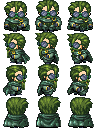
\includegraphics[width=0.3\textwidth]{example.png}
\caption{\label{fig:art} Art example of a character}
\end{figure}

\section{Forms of Engagement}
Players will be able to engage with this game in several ways. The main focus will be on the narrative experience provided as it relays the pertinent information of digital wellbeing. There will also be elements of challenge in the form of smaller challenges the player will have to face in order to progress in the game and further the story.

\
% ______________________
% chapter Game Details
% ______________________


\chapter{Gameplay and Game Setting}


\section{Story}
The game will take users through various scenarios relating to aspects of digital wellbeing which include privacy and security, mental health, physical wellbeing, etc.
\\\\
The player will encounter a specific non-player character on each level who is struggling with a certain aspect of digital wellbeing and then be tasked to gather information on that specific aspect and report it back to them.
\\\\
The story, specifically, will be:
\begin{quote}
You are a student at the NWU, lately a few of your friends and/or class mates are having troubles with technology and how they interact with it. Luckily for you, you recently met DigiBot - a robot intent on developing good relationships with technology for humans. In order to gather information on digital wellbeing, Digibot will take the player to certain area within a digital world.
\end{quote} 


\section{World/Environment}
The environment will be that of a university and surrounding areas. The player will be able to move around a specific section of the campus in each scenario. Additionally, the player may move to different areas not connected to the campus in certain scenarios, such as a "digital world" as a part of the narrative.


\section{Characters in the Game}
\begin{itemize}
\item The player character
\item DigiBot
\item Various intractable non-player characters (Friends/Classmates) 
\item "Set dressing" characters
\item Enemies
\end{itemize}

\section{Main Objective and Core Mechanics}
The objective of the game itself is to educate the player about digital wellbeing. Following this, there will be multiple objectives for each section of the game however, the overarching objective for the player is to gather some information relating to digital wellbeing for a reason the specific scenario requires.
\\\\
The core mechanics of the game are fairly simple as a player must travel around a set environment and gather information relating to some aspect of digital wellbeing. Once enough information is gathered they will be able to complete the level once they answer questions on the specific aspect for the level through some dialogue. During this final section on each level the player will be presented a question and have a selection of answers based on the information gathered and must select the correct option. If the player selects a wrong answer, DigiBot will explain what is wrong with that answer and maybe hint towards the correct answer. Following this, the player will have completed that specific level.

\section{Controls}
The game will be playable on PC/Desktop computers.
\\ 
The PC controls are as follows:
\begin{itemize}
\item The \textbf{W,S,A,D} or \textbf{Arrow} Keys for movement;
\item \textbf{Left mouse click} for selecting options in dialogue and menus; 
\item The \textbf{esc} or \textbf{Q} keys for pausing the game; and
\item Either \textbf{Spacebar} or \textbf{E} for interacting with objects or other non-player characters.
\end{itemize}


% ______________________
% chapter Front End
% ______________________
\chapter{Front End}


\section{Start Screen}

\begin{figure}[H]
\centering
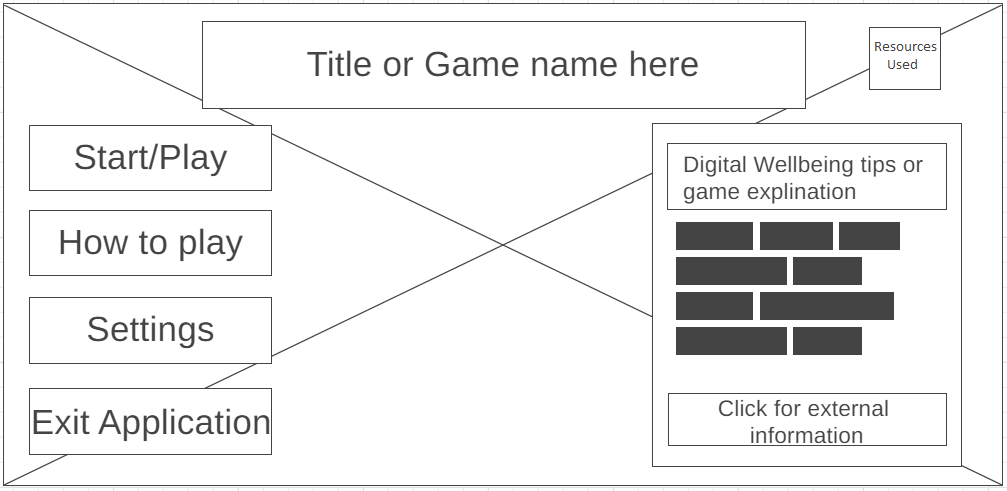
\includegraphics[width=1.1\textwidth]{TitleScreenWireFrame.PNG}
\caption{\label{fig:TS} Title Screen}
\end{figure} \noindent
This, or similar design, should work both on PC and mobile as everything is large and clear - the only issue might be that of accessibility with the explanation section on the right where text might be too small for some users.

\section{Menus}
\begin{figure}[H]
\centering
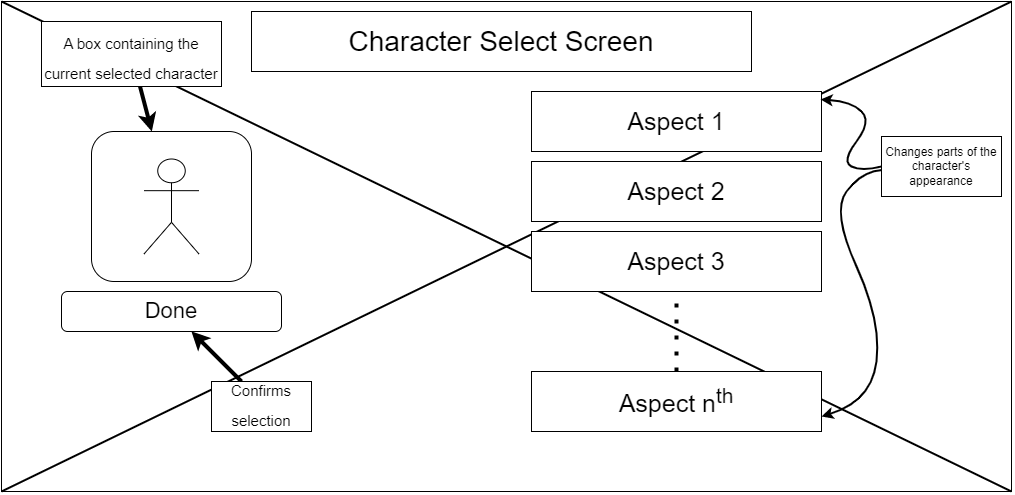
\includegraphics[width=1.1\textwidth]{CharacterSelectScreenWireFrame.png}
\caption{\label{fig:LSS} Character Selection Screen}
\end{figure}
\noindent A player is able to cycle through options for their character representation with the buttons on the right, a visible representation on the left and a confirmation button below that.

\begin{figure}[H]
\centering
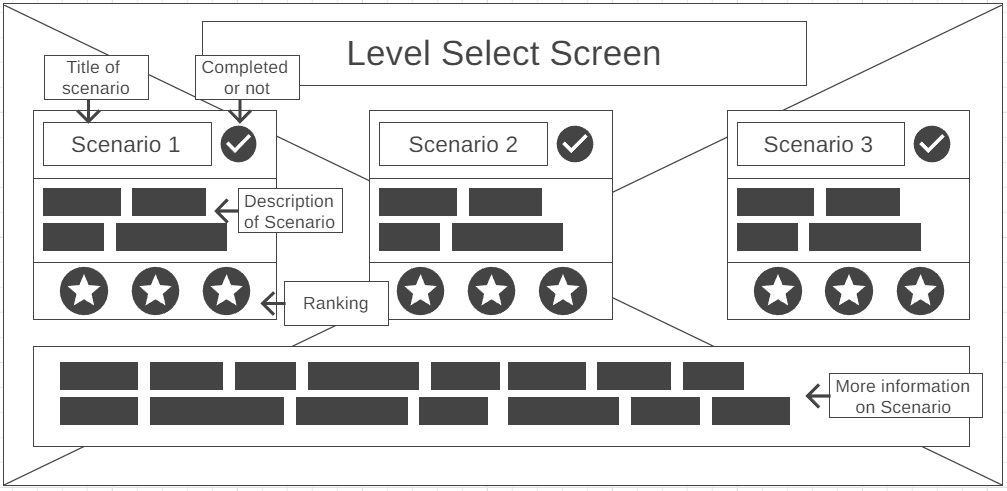
\includegraphics[width=1.1\textwidth]{LevelScreenWireFrame.PNG}
\caption{\label{fig:LSS} Level Selection Screen}
\end{figure} \noindent
This is if I go with the segmented level based approach to the SG - Space and Narrative in Computer Games in Ludotopia in the introduction talks about how open world games do not restrict players to a chronological path through the games and, with the level approach, I can have all levels unlocked at start and let users pick which one to do but, with the open world idea, users could just walk to and interact with the NPC's they wish - both approaches technically achieve the notion of player choice and freedom so....
\\\\
Additionally, with the "reach more users" research question - more platforms and modes of play means more users so might still use this regardless for the web app version as I doubt save states would be viable there as with one F5 all progress would be lost no???.


\section{End Screen}

\begin{figure}[H]
\centering
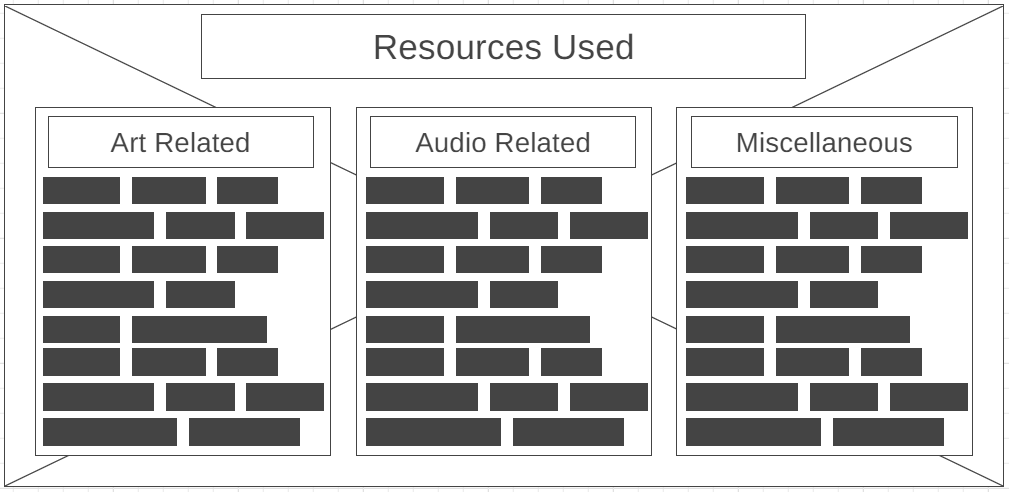
\includegraphics[width=1.1\textwidth]{ResourceScreenWireFrame.PNG}
\caption{\label{fig:RUS} Resources Used Screen}
\end{figure}
% ______________________
% chapter Game Details
% ______________________


\chapter{Technology}

\section{Target Systems}
This game is initially intended for play on PC/Desktops as a stand-alone executable and potentially in browser (albeit as a similar but different package).

\section{Hardware}
No intensive hardware required in terms of CPU and GPU specifications as it is a 2D game. An initial internet connection would be required to download the executable and a constant connection for the browser version. Additionally, some desktop system with keyboard and mouse is needed.

\section{Development Systems and Tools}
The game is being developed with the Godot game engine. Additionally, source control is accomplished using GitHub through GitHub Desktop.
\\\\
For the art tools used, most art and music will be acquired from opengameart.org and in the instances art does need to be generated and/or edited, GIMP and Aseprite are to be used.


\chapter{Timeline and Cost Estimation}

\section{Time Estimation}

\begin{figure}[h]
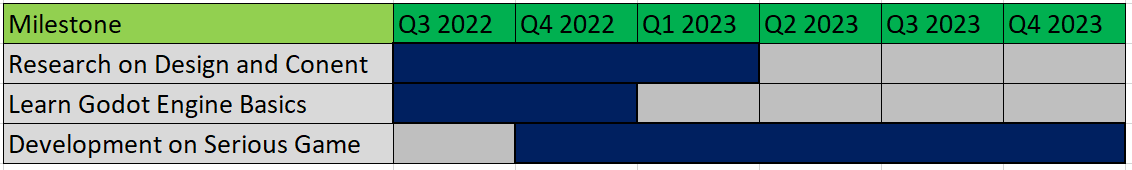
\includegraphics[scale=0.5]{gantt.PNG}
\caption{\label{fig:tl} Initial Timeline}
\end{figure}

\section{Cost Estimation}
Not Applicable. 

% ______________________
% chapter Game Details
% ______________________


\chapter{Team and Credits}
Solo developer with feedback provided by supervisors.
\\
Additional Credits (e.g. sources of art, audio,.. ) 

\section{NOTES}
Somewhat top-down pixel game where using devices moves player to a digital world of some kind 
\begin{itemize}
\item Poster idea can be implemented by having a generic poster in-game and when interacted with brings up the full version
\item Links the pysical wellbeing aspect of that one Feerrar framework nicely into the core gameplay if a "sanity-like" bar from Amnesia games is implemented
\item Have social media sections in digi-world that could increase mental health distress depending on given events
\begin{itemize}
\item ie. If major world event happens, leads to doomscrolling, worse mental health
\end{itemize}
\end{itemize}\noindent
\\
Link the physical aspects of DW to the interaction with the core design of the game
\begin{itemize}
\item have a timer to remind them of breaks and have a hard limit - have a quiz for when the user starts again - gotta add some form of active learning engagement ig
\begin{itemize}
\item have a X-min timer go off every Y-min when no action is happening for a stretch or two 
\end{itemize}
\end{itemize}\noindent
\\
Other aspects of DW are in the content of the SG 
\begin{itemize}
\item as per the top point + the sections idea can be expanded to include a security section 
\end{itemize}\noindent
\\
You are a student at the NWU, lately a few of your friends and class mates are having unhealthy/lacklustre experiences/relationships with technology. Luckily for you, you recently met DigiBot - a robot intent on developing good relationships with technology for humans - possibly for the future AI war ;P 
\begin{itemize}
\item Have game map/level layout be based on parts of campus with select areas housing a friend that needs help with  a specific aspect of digital wellbeing and near them is a portal to DigiBot's world where users will play a level designed to help understand and better that specific relationship with technology
\item Can take that quiz idea and use it when explaining to friends: 
\begin{itemize}
\item They ask a question
\item You give a response from a list
\item If right move on, else DigiBot reminds/hints towards the right answer

\end{itemize}
\item Could have DigiBot quiz the user on the way back to the portal too
\item Gameplay other than this still needs ideas... maybe a generic 2D hack'n'slash of shooter or have each section need the player to make use of the knowledge they just learned to return
\end{itemize}\noindent
\\
Users could select a player class akin to warrior, mage, etc. but instead it's stuff like secratary, programmer, etc. which  could help specify advice to each user - i.e. digital detox won't be viable for a programmer as the work requires tech
\\\\
\textbf{Since Godot uses JSON to do dialogue, it should be feasibly to have a modular system of [type of game, content of session, difficulty of session] where the "levels" could make use of all scenarios at differing difficulties. Also then ties in to the structuring of difficulty - although that would need to be on a per topic basis as having easy physical health sections and then difficult security sections doesn't work too great. Maybe have each topic have the x levels and increase the difficulty in each then}

\url{http://gameaccessibilityguidelines.com/}


%\bibliographystyle{alpha}
%\bibliography{sample}

\end{document}